\subsubsection*{例1: Basic Example}

Using the data \verb|dat1.csv|, set \verb|Age| as the unit of composition, draw a one dimensional bar graph showing the population.
The output of the bar chart can be viewed in the web browser. Note that in the bar chart, when you place the mouse cursor over the bar chart, details of the unit of composition is shown in a pop-up box. The graph can also be moved by dragging the mouse, and the size of the graph can be scaled by scrolling the mouse.


\begin{Verbatim}[baselinestretch=0.7,frame=single]
$ more dat1.csv
Age,Population
10,310504
20,552339
30,259034.5555
40,0450818
50,1231572
60,1215966
70,641667
$ mbar.rb i=dat1.csv v=Population f=Age o=result1.html
#END# /usr/bin/mbar.rb i=dat1.csv v=Population f=Age o=result1.html
$ head result1.html
<!DOCTYPE html>
<html>
<head>
<meta charset="utf-8">
<style>
body {
  font: 10px sans-serif;
}
\end{Verbatim}

\begin{flushleft}
\fbox{
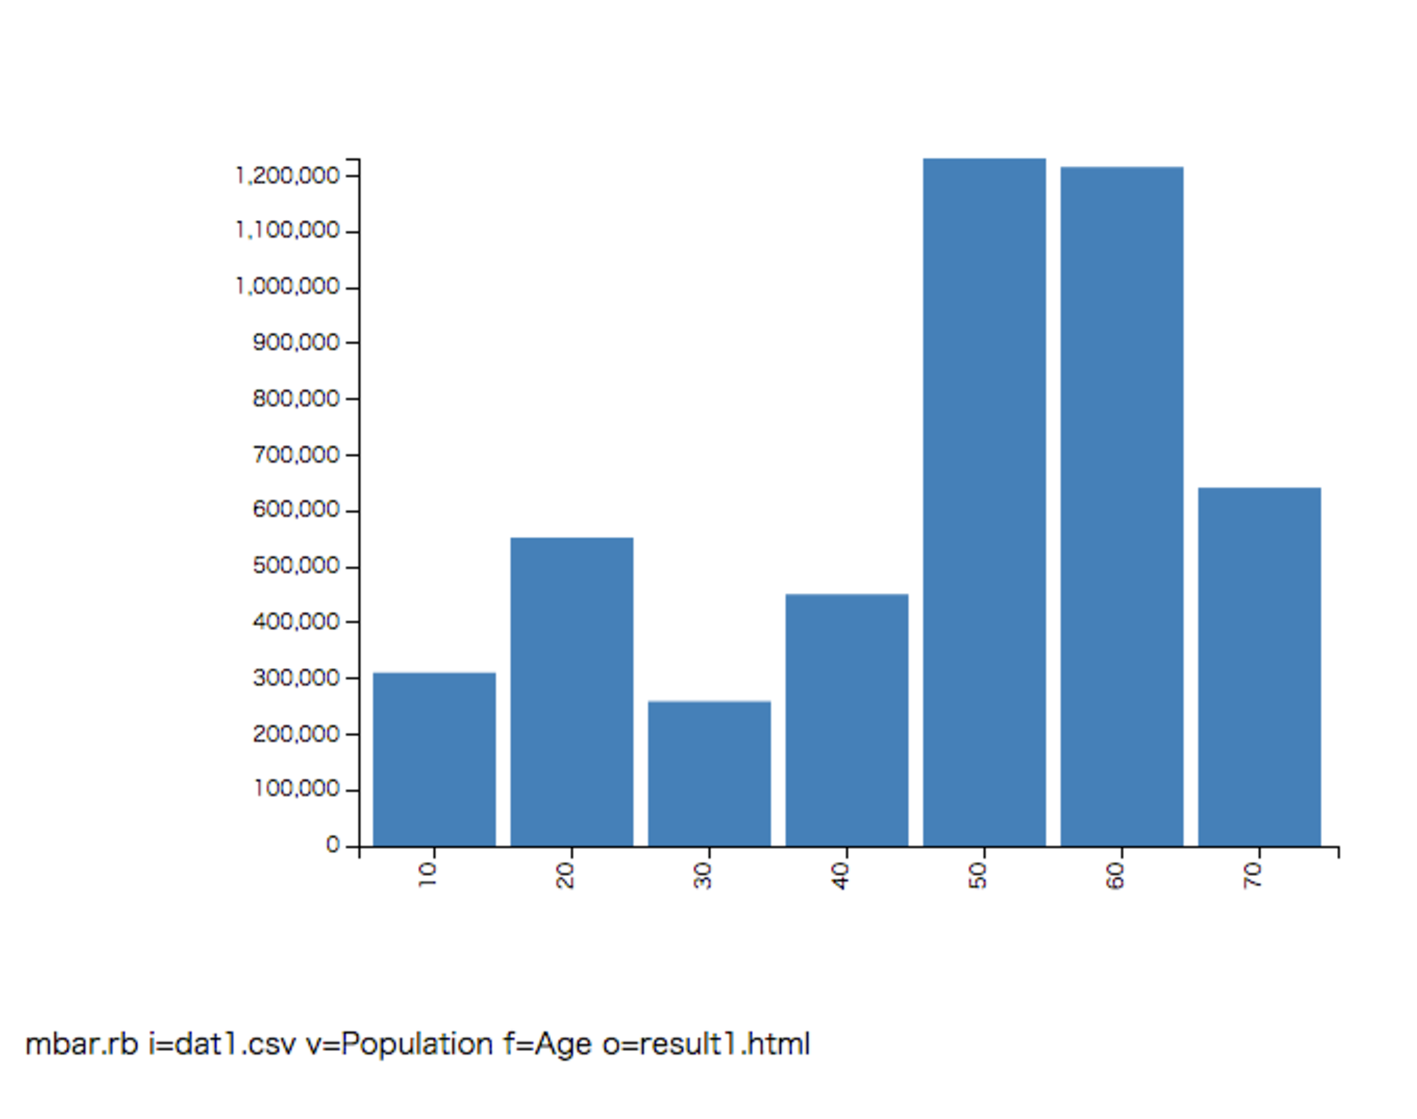
\includegraphics[scale=0.5]{figure/mbar1.eps}
}
\end{flushleft}

\subsubsection*{例2: Draw a one dimensional bar graph matrix}

Using the data \verb|dat2.csv|, set \verb|Age| as the unit of composition, draw the bar graph showing the population. Specify \verb|Pref| at ¥verb|k=| parameter, which designates pref on the x-axis, extended horizontally as a one-dimensional bar graph. Specify the title of the graph at \verb|title=| parameter.


\begin{Verbatim}[baselinestretch=0.7,frame=single]
$ more dat2.csv
Pref,Age,Population
Nara,10,310504
Nara,20,552339
Nara,30,259034
Nara,40,450818
Nara,50,1231572
Nara,60,1215966
Nara,70,641667
Hokkaido,10,310504
Hokkaido,20,252339
Hokkaido,30,859034
Hokkaido,40,150818
Hokkaido,50,9231572
Hokkaido,60,4215966
Hokkaido,70,341667
$ mbar.rb i=dat2.csv k=Pref v=Population f=Age o=result2.html title='Population of Nara and Hokkaido by Age Group'
#END# /usr/bin/mbar.rb i=dat2.csv k=Pref v=Population f=Age o=result2.html title='Population of Nara and Hokkaido by Age Group'
$ head result2.html
<!DOCTYPE html>
<html>
<head>
<meta charset="utf-8">
<style>
body {
  font: 10px sans-serif;
}
\end{Verbatim}

\begin{flushleft}
\fbox{
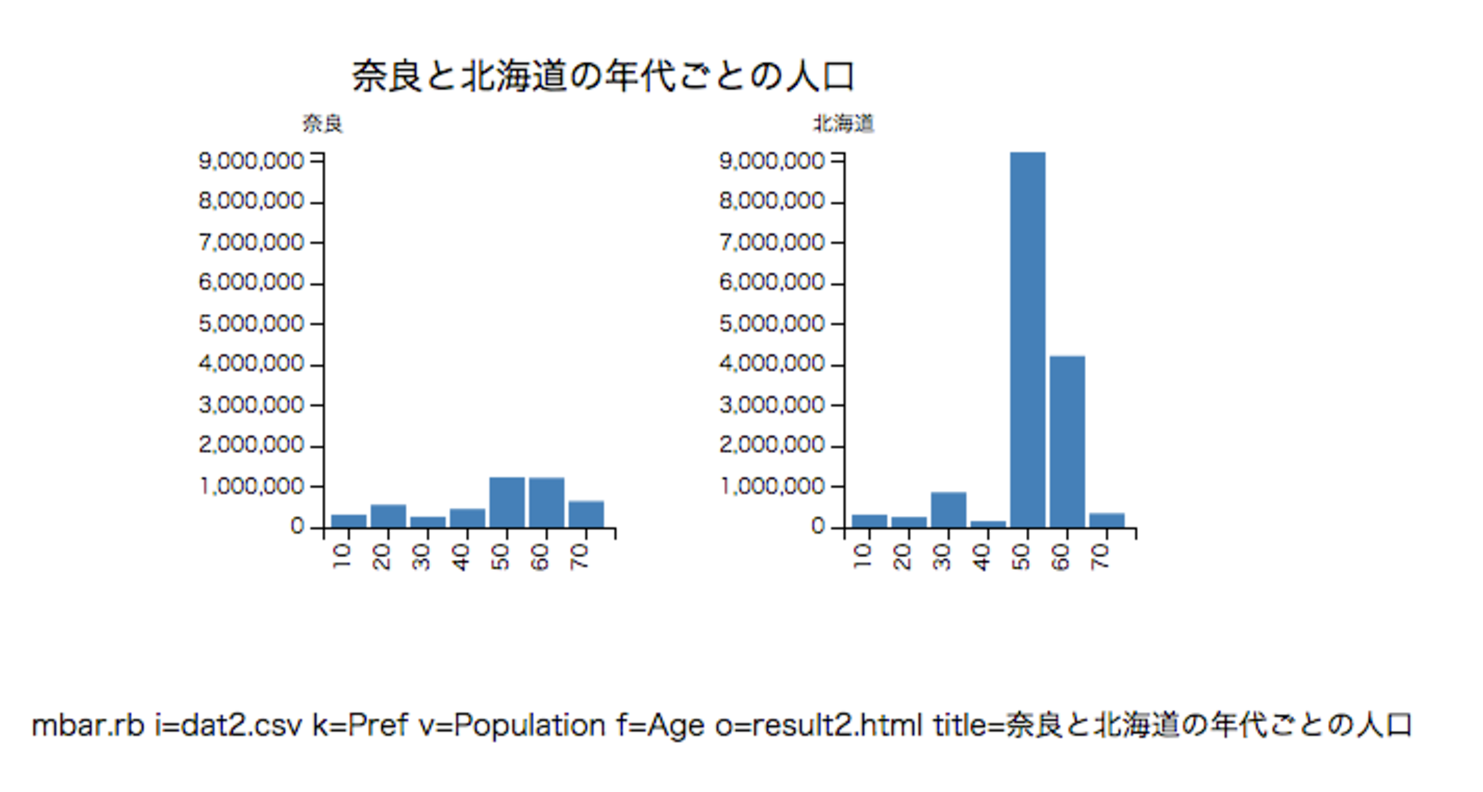
\includegraphics[scale=0.5]{figure/mbar2.eps}
}
\end{flushleft}


\subsubsection*{例3: Draw a two dimensional bar graph matrix}

Using the data \verb|dat3.csv|, set \verb|ThemePark| as the unit of composition, draw the bar graph showing the number item, and set the \verb|width=| at 200, and \verb|height=| at 150. Specify \verb|Gender| and \verb|Age| at \verb|k=| parameter, which designates Gender on the x-axis extended horizontally, and Age on y-axis extended vertically.


\begin{Verbatim}[baselinestretch=0.7,frame=single]
$ more dat3.csv
Gender,Age,ThemePark,Number
Male,30,Disney,100
Male,30,UFJ,59
Male,30,Umeyashiki,180
Male,40,Disney,200
Male,40,UFJ,3
Male,40,Umeyashiki,10
Male,50,Disney,110
Male,50,UFJ,40
Female,30,Umeyashiki,100
Female,30,Disney,80
Female,30,UFJ,200
Female,40,Disney,90
Female,40,UFJ,80
Female,40,Umeyashiki,120
Female,50,Disney,99
Female,50,UFJ,80
Female,50,Umeyashiki,110
$ mbar.rb i=dat3.csv k=Gender,Age v=Number f=ThemePark o=result3.html
#END# /usr/bin/mbar.rb i=dat3.csv k=Gender,Age v=Number f=ThemePark o=result3.html
$ head result3.html
<!DOCTYPE html>
<html>
<head>
<meta charset="utf-8">
<style>
body {
  font: 10px sans-serif;
}
\end{Verbatim}

\begin{flushleft}
\fbox{
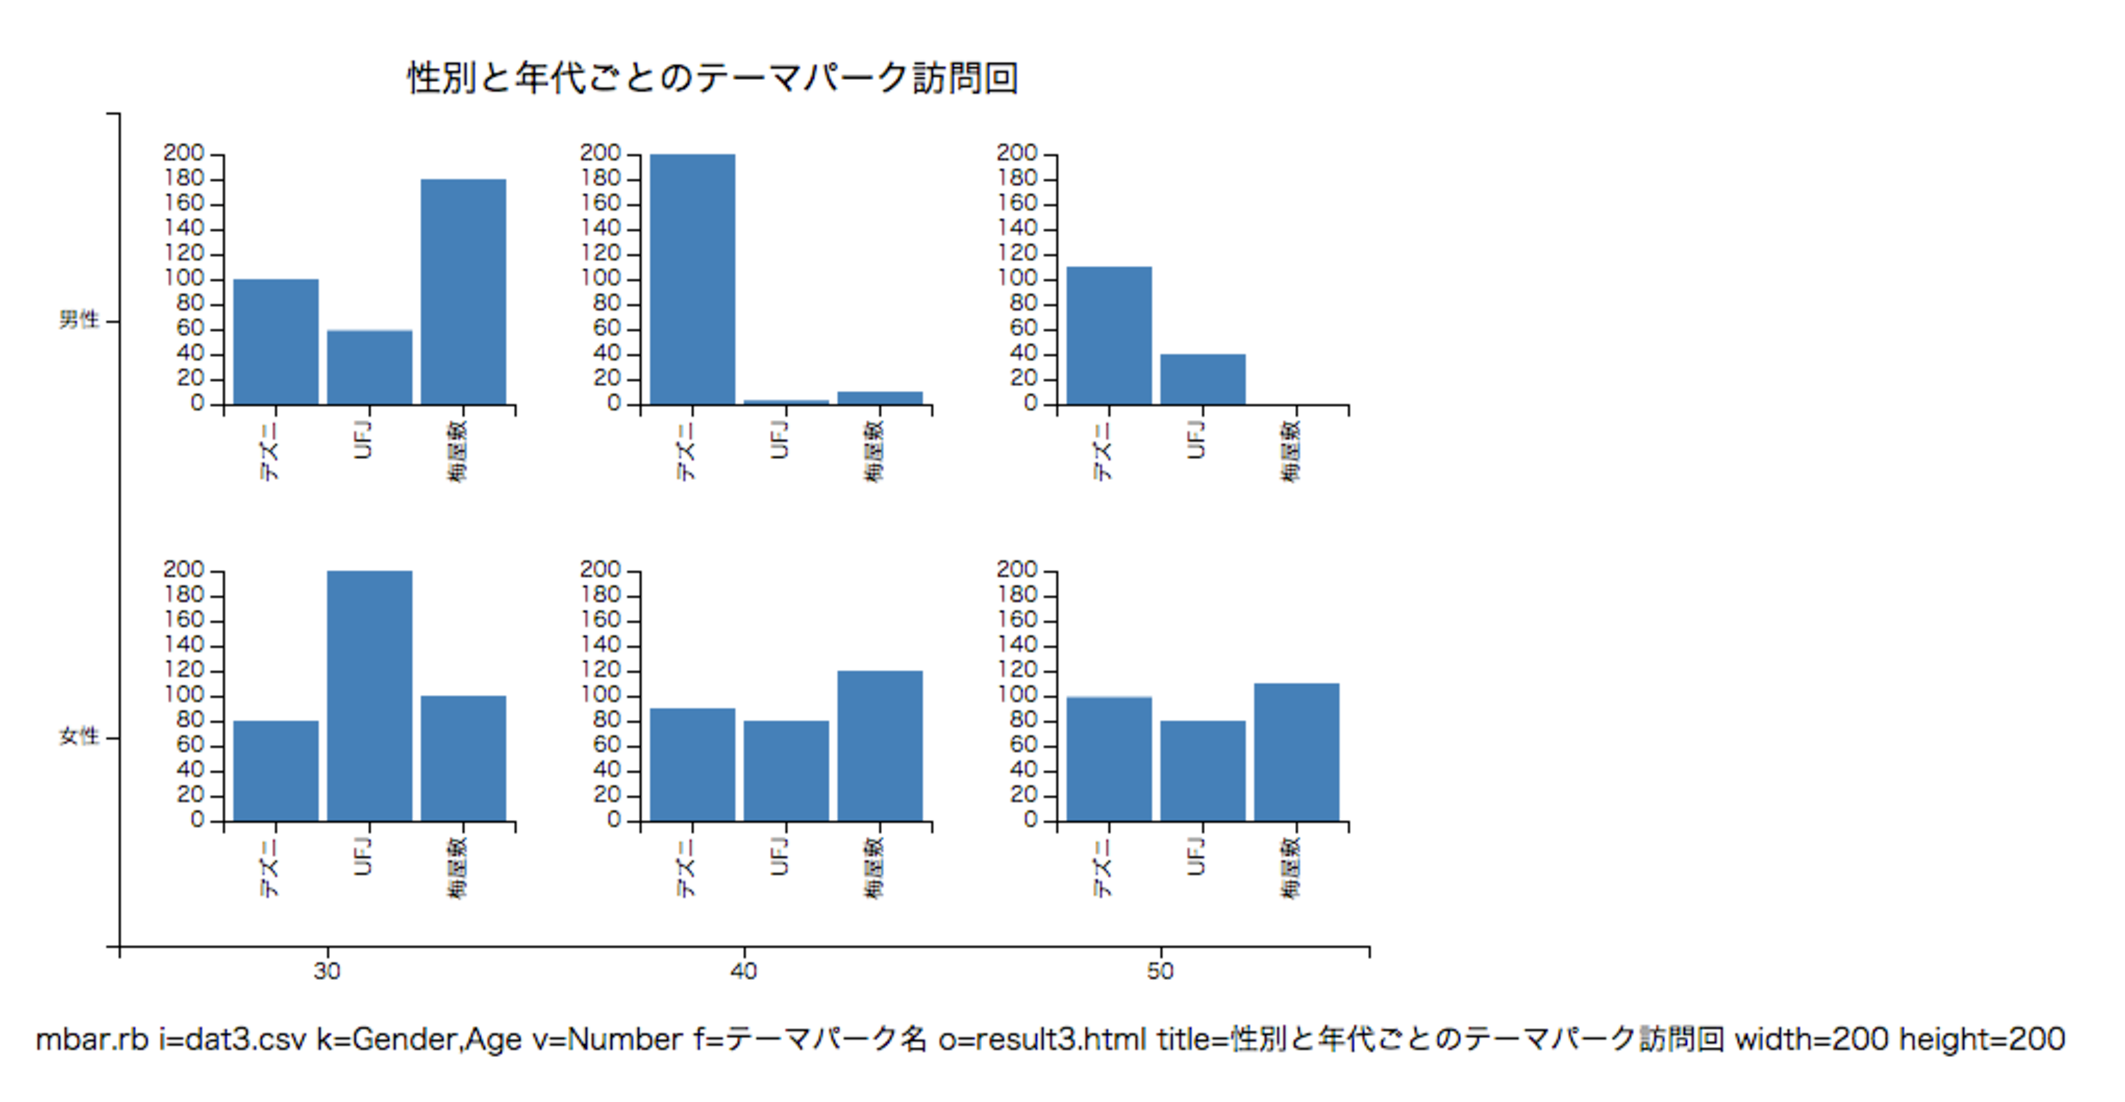
\includegraphics[scale=0.5]{figure/mbar3.eps}
}
\end{flushleft}

